\section{Architecture}\label{sec:Architecture}

% Describe the data processing pipeline here. 
% 1. Get the raw data and remove the ground (LiDAR data clean up)
% 2. Segment data and sent it to classifier 
% 3. Classification with Neural Network. 


Our data processing pipeline consist of 3 main processing steps: 

\begin{enumerate}
  \item \textbf{Step-1  Filtering. } Filtering the LiDAR base lines (cylinder lines around objects - See Figures \ref{fig:ground_before} and \ref{fig:after})
  \item \textbf{Step-2 Object Segmentation.} Separating the 3D point cloud to segments that contain one single object or in other words marking the object with a voxel grid.  
  \item \textbf{Step-3 Object Classification.}  Sending data of a single object to classifier for classification.  
\end{enumerate}


Figure \ref{fig:dataPipeline} depicts our data processing pipeline. As the system runs in the testing time in gets point cloud data for a single scene which includes multiple objects and process it in 3 steps and to deliver the classification results in real-time.   

The provided training data by DEBS 2019 Challenge \cite{DEBSGC2019} includes only one single object per scene with its label so that it is not require to have the step-2 object segmentation when we train our system.


\begin{figure*}[ht!]
 \begin{center}
   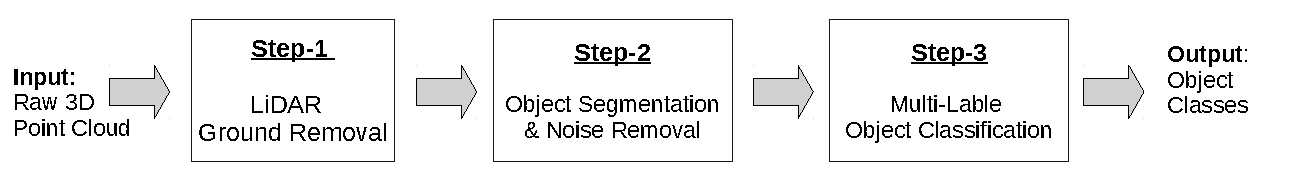
\includegraphics[width=0.9\textwidth]{./images/DataProcessingPipleline.pdf}
   \caption{An Overview of our Data Processing Architecture}
   \label{fig:dataPipeline}
 \end{center}
\end{figure*}




% Describe \ldots. 
% 
% Different forms of data processing architectures that we have implemented and tested . 
% 
% \begin{enumerate}
%   \item Different methods for removing noise from raw data (data preprocessing). 
%   \item Projecting 3D data into 2D data using 3 different projection methods 
%   \item CNN  (with and without maxpool) + fully-connected + dropout + fully-connected+softmax
%   \item CNN with different number of hidden layers. 
% 
% \end{enumerate}



% KIA
% We need another image to describe the CNN architecture. 
% Add two images about it. 




\subsection{LiDAR Ground Data Removal}
% Describe here how we remove the ground - keep this very general 
% 

The first step in our data processing pipeline is to filter out the LiDAR laser lines that are building a cylinder form 3D shape from the laser standing point $(x=0, y=0, z=0)$. Figure \ref{fig:ground_before} visualizes the LiDAR data from a single scene with LiDAR laser lines and Figure \ref{fig:after} shows the data after filtering the Laser ground lines. As you can see objects like car or pedestrian are visible in Figure \ref{fig:after} after filtering the LiDAR lines.

This first filtering step in our data processing pipeline reduces highly the amount of data that we process and also heps to be able to find object segments in the next following step. 
We training and test the classification model (in the Step-3) after removing the Laser base lines and filtering them out.  


\begin{figure*}[!ht]
\centering
\begin{minipage}{0.49\textwidth}
  \centering
        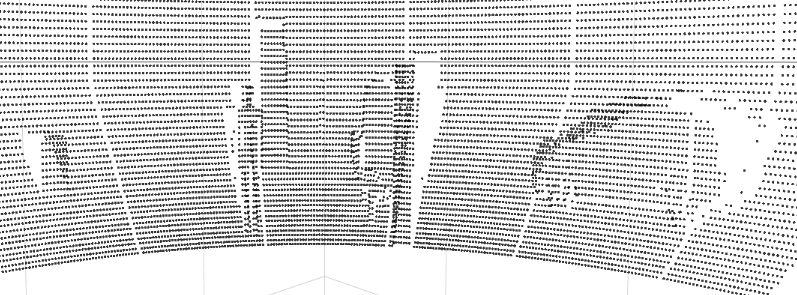
\includegraphics[width=.9\linewidth]{images/ground_before2.png}
        \caption{LiDAR Raw Point Cloud Data}
        \label{fig:ground_before}
\end{minipage}%
\begin{minipage}{0.49\textwidth}
  \centering
        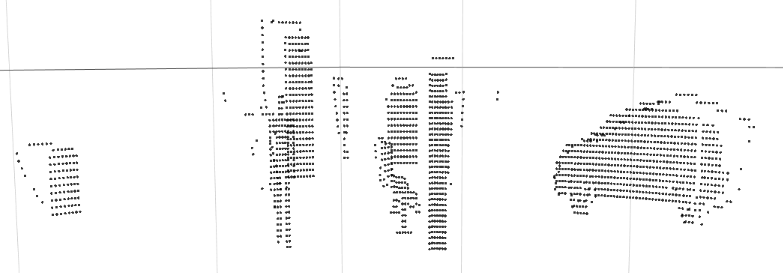
\includegraphics[width=.9\linewidth]{images/ground_after2.png}
        \caption{Data After Filtering the LiDAR Scan Lines (Ground)}
        \label{fig:after}
\end{minipage}%
% \caption{General caption.} \label{fig:1}
\end{figure*}


% Describe here how we filter the ground. 



\subsection{Object Segmentation and Noise Removal}






%\usepackage{graphics} is needed for \includegraphics
\begin{figure*}[!ht]
\begin{center}
  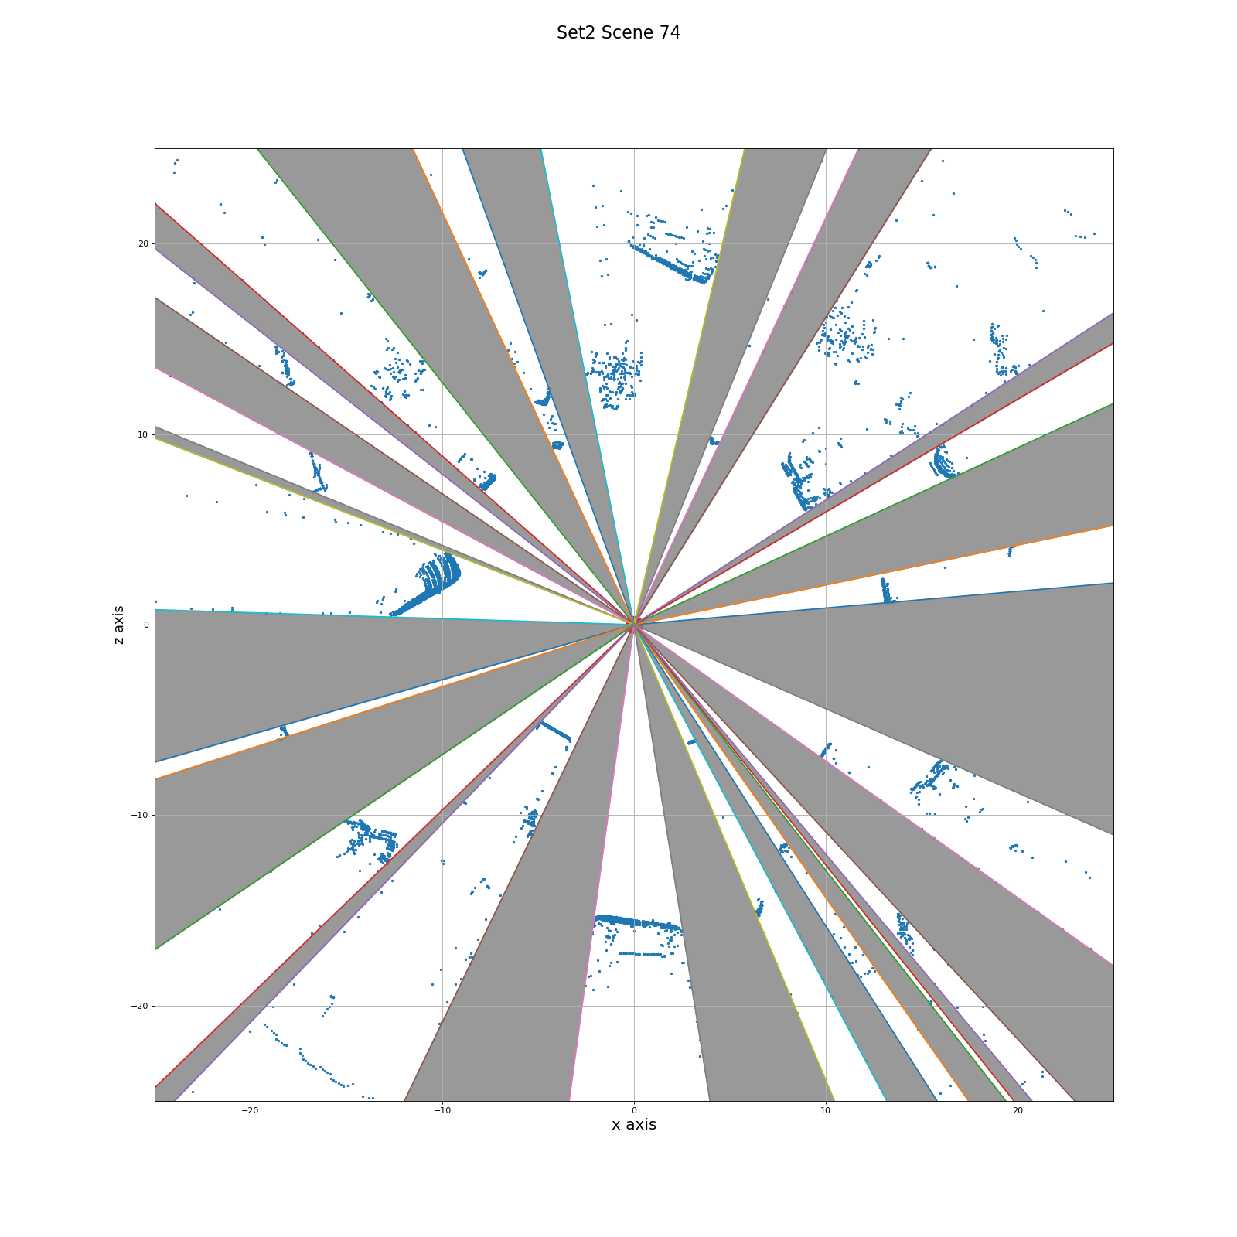
\includegraphics[scale=0.5]{./images/sector-with-bg/74.pdf}
  \caption{Top-View - Unoccupied Sectors (gray colored) and  Sectors including objects}
  \label{fig:sectors}
\end{center}
\end{figure*}







